\documentclass{ieeeaccess}
\usepackage{cite}
\usepackage{amsmath,amssymb,amsfonts}
\usepackage{algorithmic}
\usepackage{graphicx}
\usepackage{textcomp}
\usepackage{booktabs}
\usepackage{multirow}
\usepackage{xcolor}
\usepackage{url}

% 中文支持（中文先行草稿阶段使用 xelatex 编译）
% 最终英文投稿版改回 pdflatex 并删除 xeCJK 相关行
\usepackage{xeCJK}
\setCJKmainfont{STSong}
\setCJKsansfont{STHeiti}
\setCJKmonofont{STFangsong}

\usepackage{bm}
\makeatletter
\AtBeginDocument{\DeclareMathVersion{bold}
\SetSymbolFont{operators}{bold}{T1}{times}{b}{n}
\SetSymbolFont{NewLetters}{bold}{T1}{times}{b}{it}
\SetMathAlphabet{\mathrm}{bold}{T1}{times}{b}{n}
\SetMathAlphabet{\mathit}{bold}{T1}{times}{b}{it}
\SetMathAlphabet{\mathbf}{bold}{T1}{times}{b}{n}
\SetMathAlphabet{\mathtt}{bold}{OT1}{pcr}{b}{n}
\SetSymbolFont{symbols}{bold}{OMS}{cmsy}{b}{n}
\renewcommand\boldmath{\@nomath\boldmath\mathversion{bold}}}
\makeatother

\def\BibTeX{{\rm B\kern-.05em{\sc i\kern-.025em b}\kern-.08em
    T\kern-.1667em\lower.7ex\hbox{E}\kern-.125emX}}

% TODO 标记宏
\newcommand{\TODO}[1]{\textcolor{red}{\textbf{[TODO: #1]}}}

%% ============================================================
\begin{document}
% 草稿占位：投稿时由 IEEE 分配，格式沿用官方模板默认值
\doi{10.1109/ACCESS.2026.DOI}
\vol{PREPRINT}
\year{2026}

\title{Temporal Pixel Masking for Reducing OCR Recovery from Short-Exposure Screen Photographs: A Single-UVC-Camera Feasibility Study}

\author{\uppercase{First A. Author}\authorrefmark{1}
\TODO{作者信息待填}}

\address[1]{\TODO{单位地址待填}}

\tfootnote{\TODO{基金致谢待填}}
% 英文终稿伦理脚注（机构无伦理委员会时的 IEEE 规范句式，翻译时并入上面的 \tfootnote）：
% ``This work involved human subjects in its research. The authors' institution
% does not maintain an ethics review board for minimal-risk behavioral studies
% of this type; all procedures followed the informed-consent and safety protocol
% described in Section V-D.''

\markboth
{Author \headeretal: Temporal Pixel Masking Against Short-Exposure Screen Photography}
{Author \headeretal: Temporal Pixel Masking Against Short-Exposure Screen Photography}

\corresp{Corresponding author: \TODO{通讯作者邮箱}.}

%% ============================================================
%% 摘 要
%% ============================================================
\begin{abstract}
智能手机或智能眼镜可静默拍摄屏幕，再经光学字符识别（OCR）或视觉语言模型提取文字。本文利用观察者与相机在时间积分上的差异，以~CSPRNG~驱动的随机过程将每帧拆成高速交替的互补子帧：观察者跨子帧整合可读内容，短曝光相机则主要记录残缺像素。在单一~USB~视频类（UVC）网络相机、9~组距离/角度共~10\,575~次采集的可行性实验中，短曝光条件下逐样本最强~OCR~字符恢复率由未保护的~94.1\%~降至可读优先档（deployed profile）的~15.1\%~和抗拍强化档（capture-hardened profile）的~5.0\%，完全匹配率由~65.7\%~分别降至~0.4\%~和~0\%。不过，抗拍强化档在视频时域平均下仍有~47.9\%~字符恢复率；三个商用视觉语言模型也能从大字号短片段的短曝光照片中恢复可观文本。有效性主张限于所测~UVC~链路中传统~OCR~的短曝光缓解，不覆盖其他相机、完整周期积分或现代视觉语言模型。可读性与舒适度由色差、SSIM~等数字代理指标描述，计划中的用户研究尚未开展，实际体验有待验证。
\end{abstract}

\begin{keywords}
adversarial perturbation, anti-photography, camera capture, display privacy, OCR, persistence of vision, temporal masking, visual eavesdropping
\end{keywords}

\titlepgskip=-21pt
\maketitle

%% ============================================================
%% I. 引 言
%% ============================================================
\section{引言}
\label{sec:introduction}

\PARstart{S}{creens} 屏幕遍及办公、金融、医疗、会议等场景，而智能手机、智能眼镜（如~Ray-Ban Meta）~\cite{b_wang2026}~和微型相机同样随处可见。攻击者只需拍一张屏幕照片，即可用~OCR~提取文字或用目标检测识别界面元素。这种”视觉窃听”（visual eavesdropping）隐蔽且成本极低，不留网络入侵痕迹，也无需物理接触设备；受控实验与实地调研均表明其在日常场景中普遍存在且成功率高~\cite{b_ponemon2016,b_eiband2017}。本文以上述设备作为威胁动机，但当前物理证据仅覆盖单一~UVC~网络相机下的屏--相机链路；手机、智能眼镜和其他相机~ISP~管线的复现性留待后续验证。

\subsection{现有方案及其不足}

现有屏幕隐私防护方案各有适用边界。物理隐私膜（如商业防窥膜）只限制可视角度，无法阻止正对相机的拍摄。软件层的被动画质退化（调暗、模糊、像素化）以牺牲全局可读性或依赖观察几何为代价，难以针对性阻断正面抓拍（数值对比见~\S\ref{sec:simulation}）。数字水印仅提供事后追责能力~\cite{b_fang2019}。面向影视防盗录的时域重编码方案（如~Kaleido~\cite{b_kaleido2015}）旨在退化连续录像观感，未涉及静态敏感内容的短曝光单帧抓拍与机器识别（\S\ref{sec:related}）。上述方案分别覆盖视角限制、事后追踪和连续录像干扰，而正对相机的短曝光抓拍及机器识别恰好落在空白地带。

对相机施加信息退化往往也会降低合法用户的可读性。本文探讨能否利用显示的时间结构，在短曝光拍摄场景中拉开二者差距。

\subsection{核心思想}

本文利用观察者时间整合与相机曝光窗口之间的差异：将每帧画面在时域上拆成~$n$~个随机互补子帧高速交替显示。曝光时间短于或接近一个子帧时，相机主要记录不完整的像素子集，观察者则跨多个子帧整合内容（图~\ref{fig:concept}）。但相机曝光并非瞬时采样，长曝光或视频重构覆盖完整周期时互补子帧可被重新累加，故本文不对任意曝光条件作不可恢复的保证。

本文将短曝光建模为机会性拍摄的首要攻击层级：攻击者在不校准曝光、不持续对准屏幕的情况下快速抓拍一张照片。这不等于主张所有默认智能手机都会选择子帧级快门：S600~实验使用的是固定校准曝光而非手机自动曝光。能力更强的攻击者可刻意延长积分时间或录制视频，这些模式是更高层级的攻击与安全边界，而非被排除的特例。

\begin{figure}[!t]
\centering
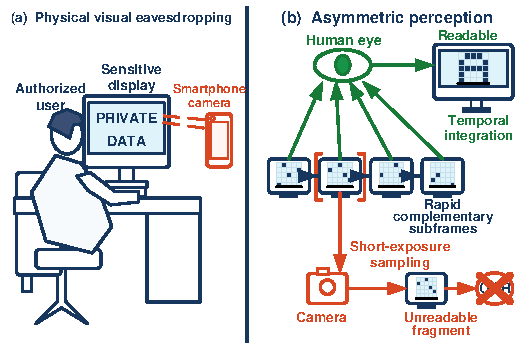
\includegraphics[width=\columnwidth,viewport=0 0 252 168,clip]{figures/visio/figure1_concept_threat/final/figure1_concept_threat.pdf}
\caption{威胁场景与时域像素掩模的运行边界。(a)~附近相机可在无主机系统访问权限的情况下拍摄屏幕敏感内容。(b)~人类视觉会整合互补子帧，而相机的短曝光可能仅捕捉显示周期的一部分，留给~OCR~不完整的片段。相机的图示路径仅为概念性说明：它不假设采样时间为零，也不假设人类有固定的积分时间；长曝光或多帧重构能够恢复实质性更多的信息。}
\label{fig:concept}
\end{figure}

\subsection{贡献}

主要贡献如下：
\begin{enumerate}
\item 在既有时间掩模思想基础上，实现面向传统~OCR~短曝光抓拍的时域像素掩模：CSPRNG~驱动的像素级互补子帧、可选互补对抗噪声和~GPU~渲染原型。有效性取决于相机曝光窗口与攻击者的识别管线。

\item 使用一款~eMeet SmartCam S600 USB~网络相机，在~3~个距离~$\times$~3~个角度下完成~10\,575~次真机采集的可行性验证。该语料由组件消融、参数扫描和攻击评测构成，非平衡全因子设计；主要有效性结论取自核心短曝光~OCR~子集：可读优先档字符恢复率~15.1\%（精确匹配~0.4\%），抗拍强化档~5.0\%（精确匹配~0\%）。

\item 在~OCR~主实验之外，以~4~个目标检测器（COCO~val2017，150~张真机图像加~8~张仿真诊断图像）、MOT17~关联评测（5\,316~帧仿真、450~帧真机停帧）和~3~个商用~VLM（0$^{\circ}$~轴向三个距离）作为跨任务压力测试与攻击边界探针。VLM~实验提供的是负面边界证据：传统~OCR~防护不能自动转化为端到端视觉识别防护。

\item 量化积分攻击下的残余泄漏：数字模拟中理想完整周期积分可恢复~95.2\%，真机视频时域平均对可读优先档仍恢复~71.1\%~字符。抗拍强化档将真机视频泄露降至~47.9\%~字符/5.6\%~精确匹配率，但该类攻击仍是根本性边界。真机~VLM~探针显示大字号短文本的短曝光防护在现代~VLM~面前失效：0.5\,m~处~Qwen3-VL~精确匹配达~77.8\%，1.5\,m~处三款模型仍有~33.3--47.2\%。

\item 报告~FPI、$\Delta E$、SSIM~等代理指标和~Pareto~前沿，区分数字积分代理与实际用户体验，并为后续可用性验证设计了受控组内实验协议。
\end{enumerate}

后续结构：\S\ref{sec:related}~回顾相关工作，\S\ref{sec:threat}~定义攻击者层级与防护目标，\S\ref{sec:method}~介绍掩模设计，\S\ref{sec:evaluation}~报告评估实验，\S\ref{sec:discussion}--\ref{sec:conclusion}~讨论部署边界并总结全文。


%% ============================================================
%% II. 相关工作
%% ============================================================
\section{相关工作}
\label{sec:related}

\subsection{屏幕视觉窃听威胁}

已有文献记录了多种屏幕窃取途径：远距离屏幕阅读（望远镜、长焦镜头）~\cite{b_backes2009}、HDMI~电磁泄漏的深度学习重建~\cite{b_fernandez2024}、智能眼镜隐蔽拍摄~\cite{b_wang2026}、反射/折射间接窃取~\cite{b_raguram2011}。Ponemon~Institute~的受控实验显示~91\%~的视觉窃听尝试可在~15~分钟内成功~\cite{b_ponemon2016}；Eiband~等~\cite{b_eiband2017}~通过~174~人实地调研揭示了肩窥在日常环境中的普遍性。Tang~和~Shin~\cite{b_tang2023}~提出~Eye-Shield，用前置摄像头检测旁观者并实时模糊敏感区域，但依赖用户端硬件且仅做局部遮蔽。本文聚焦不要求拍摄端合作的显示侧缓解机制，但不声称在所有曝光和重构条件下均能阻止信息获取。

\subsection{显示隐私保护}

物理隐私膜通过限制可视角度阻挡侧面偷窥，但无法阻止正对相机。Chen~等~\cite{b_hidescreen2019}~提出~HideScreen，对敏感区域做网格渲染以抑制低频线索，使内容在设定距离外与背景融合，目标是空间域防肩窥，不涉及短曝光相机抓拍或机器识别。Zhu~等~\cite{b_zhu2017}~提出~LiShield，用智能~LED~调制照明干扰滚动快门相机成像，但作用于环境光源而非显示内容。视觉密码术将秘密图像分拆为多份叠加还原~\cite{b_naor1994}，启发了时域分拆思路，但原始方案面向打印介质。数字水印~\cite{b_zhong2023}~可嵌入追踪标识，近年已有抗屏摄鲁棒变体~\cite{b_fang2019}，但本质上提供事后溯源而非事前阻断。软件防截屏（DRM）仅防数字截图，不防物理拍摄。

屏-相机可见光通信（screen-camera VLC）~\cite{b_nguyen2016,b_tran2021,b_ghiasi2024}~同样利用人眼时间积分，在画面中嵌入人眼不可见的信息供相机解码。本文与之互为”镜像”：VLC~让相机\emph{读取}隐藏信息，本文则让相机\emph{无法}读取显示内容。

Yerazunis~和~Carbone~\cite{b_yerazunis2001}~最早提出利用图像时间掩模增强显示隐私。Wu~和~Zhai~\cite{b_wu2013}~系统化了时域心理视觉调制，Gao~等~\cite{b_gao2014}~将其用于信息安全显示。Zhang~等~\cite{b_kaleido2015}~的~Kaleido~在标准刷新率屏幕上对视频帧作多帧重编码，利用屏--眼与屏--相机通道差异使影片”可看不可录”；Yang~等~\cite{b_rainbow2018}~的~Rainbow~延续该方向，覆盖移动相机拍摄。这类方案以破坏连续录像观感为目标，评测使用~PSNR、SSIM~和主观评分，与本文关注的~OCR、检测和~VLM~机器恢复率不可互替，也均未涉及静态内容的短曝光单帧抓拍与机器识别。机制上，Kaleido~的分解在连续颜色空间中进行，以色度互补帧配合亮度变化降低录像观感，依赖周期内面向人眼的完备混合；本文则采用~CSPRNG~驱动的离散像素级互斥分片，抗拍强化档主动放弃严格完备性以对抗积分攻击（\S\ref{sec:hardened}）。Lim~\cite{b_lim2007}~利用视觉暂留在浏览器中生成防截屏键盘，使单次截屏只得到局部图案。时域分片本身并非本文首创，本文的增量在于：（1）面向物理相机传统~OCR~短曝光抓拍的像素级~CSPRNG~互补分片与强化档实现；（2）单~UVC~摄像头~9~组几何条件下~10\,575~次真机采集，核心短曝光~OCR~子集作为可行性证据；（3）目标检测、关联和~VLM~探针作为跨任务压力测试而非通用视觉防护证明；（4）对完整周期平均和~VLM~失守的定量边界分析。

\subsection{对抗扰动与物理世界鲁棒性}

数字域对抗扰动~\cite{b_goodfellow2015,b_madry2018,b_carlini2017}和物理世界对抗补丁~\cite{b_eykholt2018,b_thys2019,b_xu2020}已有广泛综述~\cite{b_wei2024}。Athalye~等~\cite{b_athalye2018}~通过~EoT~实现了首个跨视角鲁棒的~3D~物理对抗物体，但仍依赖白盒目标模型。数字到物理的跨域鲁棒性差距明显：像素级扰动经相机采样和~JPEG~压缩后大幅削弱~\cite{b_eykholt2018}；物理补丁虽具跨视角鲁棒性，但需针对特定分类器生成图案~\cite{b_thys2019,b_xu2020}，对未知模型迁移性有限~\cite{b_zhao2023}。屏-相机链路还会引入摩尔纹等光学伪影，Niu~等~\cite{b_niu2021}~证明其本身即可充当对抗扰动。本文不在内容上加扰动，而在时域显示层做分片掩模——物理拍摄天然是”采样”过程，防御嵌入显示本身，无需假设攻击者使用何种识别模型。


%% ============================================================
%% III. 威胁模型
%% ============================================================
\section{威胁模型}
\label{sec:threat}

\subsection{保护资产}

屏幕上显示的敏感文字和视觉信息：密码、金融数据、个人身份信息（PII）、代码、机密文档等。

\subsection{攻击者能力}

攻击能力并非单调等级，而由曝光、几何条件、时间采样和后处理能力共同决定。本文按以下范围报告结果：
\begin{itemize}
\item \textbf{主要防护范围}：传统~OCR~攻击者的机会性短曝光快照。曝光时间短于或接近一个子帧时长；攻击者可选择~OCR~引擎，但不具备覆盖完整周期的观测数据。该层级对应无曝光校准、无持续瞄准的快速单次抓拍，并非最强理性攻击者。
\item \textbf{评测边界}：长曝光、视频时域平均、离轴拍摄、已知周期后的相位搜索与通道重构、目标检测/关联任务、商用~VLM~的端到端识别（\S\ref{sec:vlm}）。本文量化了上述攻击或迁移风险，仅将抗拍强化档的结果解释为缓解，不保证完全阻断。
\item \textbf{尚未覆盖}：更多相机/显示器组合、卷帘快门行对齐、真实世界时域超分辨率、针对显示序列训练的学习型重构器，以及长期自适应攻击。
\end{itemize}

\subsection{攻击者知识}

攻击者\emph{已知}时域掩模算法、子帧数~$n$~和候选周期参数，\emph{未知}当前周期的掩模种子和相位起点。CSPRNG~用于避免固定空间图案和跨周期重复，不提供防范完整周期平均的密码学保证——一旦攻击者获得并配准完整周期，未知种子无法阻止线性重构。

\subsection{防护目标}

短曝光条件下的分层设计目标按档位设定：抗拍强化档以传统~OCR~字符恢复率~$<5\%$~且精确匹配率~$=0\%$~为严格达标线；可读优先的~deployed~档以字符恢复率相对未保护基线降幅~$\geq80\%$~且精确匹配率~$<1\%$~为目标。目标检测的~mAP50~变化用于探索跨任务迁移风险，不作为主要达标标准。上述阈值指导参数选择与档位权衡，不构成对所有攻击模式的形式化安全保证；VLM~攻击者的结果不纳入达标判定，作为安全边界单独报告（\S\ref{sec:vlm}）。可用性方面，FPI、$\Delta E$~和~SSIM~用作代理指标；用户研究尚未开展，本文不据此声称”人眼无感”。


%% ============================================================
%% IV. 方法
%% ============================================================
\section{系统设计}
\label{sec:method}

\subsection{时域子帧分解}

给定归一化原始帧~$\mathbf{I}\in[0,1]^{H\times W\times C}$，生成二值掩模~$\mathbf{M}_1,\ldots,\mathbf{M}_n$，满足~$\sum_{k=1}^{n}\mathbf{M}_k=\mathbf{1}$，令~$\mathbf{I}_k=\mathbf{I}\odot\mathbf{M}_k$，则：
\begin{itemize}
\item \textbf{数字域完备性}：$\sum_{k=1}^{n}\mathbf{I}_k = \mathbf{I}$；
\item \textbf{互斥性}：每个像素在~$n$~个时隙中恰好被点亮一次
\end{itemize}
“求和”与”时间平均”需加区分。在等时长、等峰值亮度的理想线性显示上，一个周期的平均辐亮度为~$\mathbf{I}/n$~而非~$\mathbf{I}$。数字域完备性说明子帧可被重新求和，不等价于真实显示亮度已无损恢复。

掩模生成采用~ChaCha20~\cite{b_chacha2008} CSPRNG~和~Fisher--Yates~置换~\cite{b_knuth1997}，将每个像素随机分配至一个子帧；实现中对生成的时隙计数做卡方均匀性检查，未通过则重新采样种子。随机种子降低固定图案和跨周期相关性，但不改变完整周期可被线性求和这一事实。图~\ref{fig:pipeline}~展示从原始帧到子帧显示的管线。

\begin{figure*}[!t]
\centering
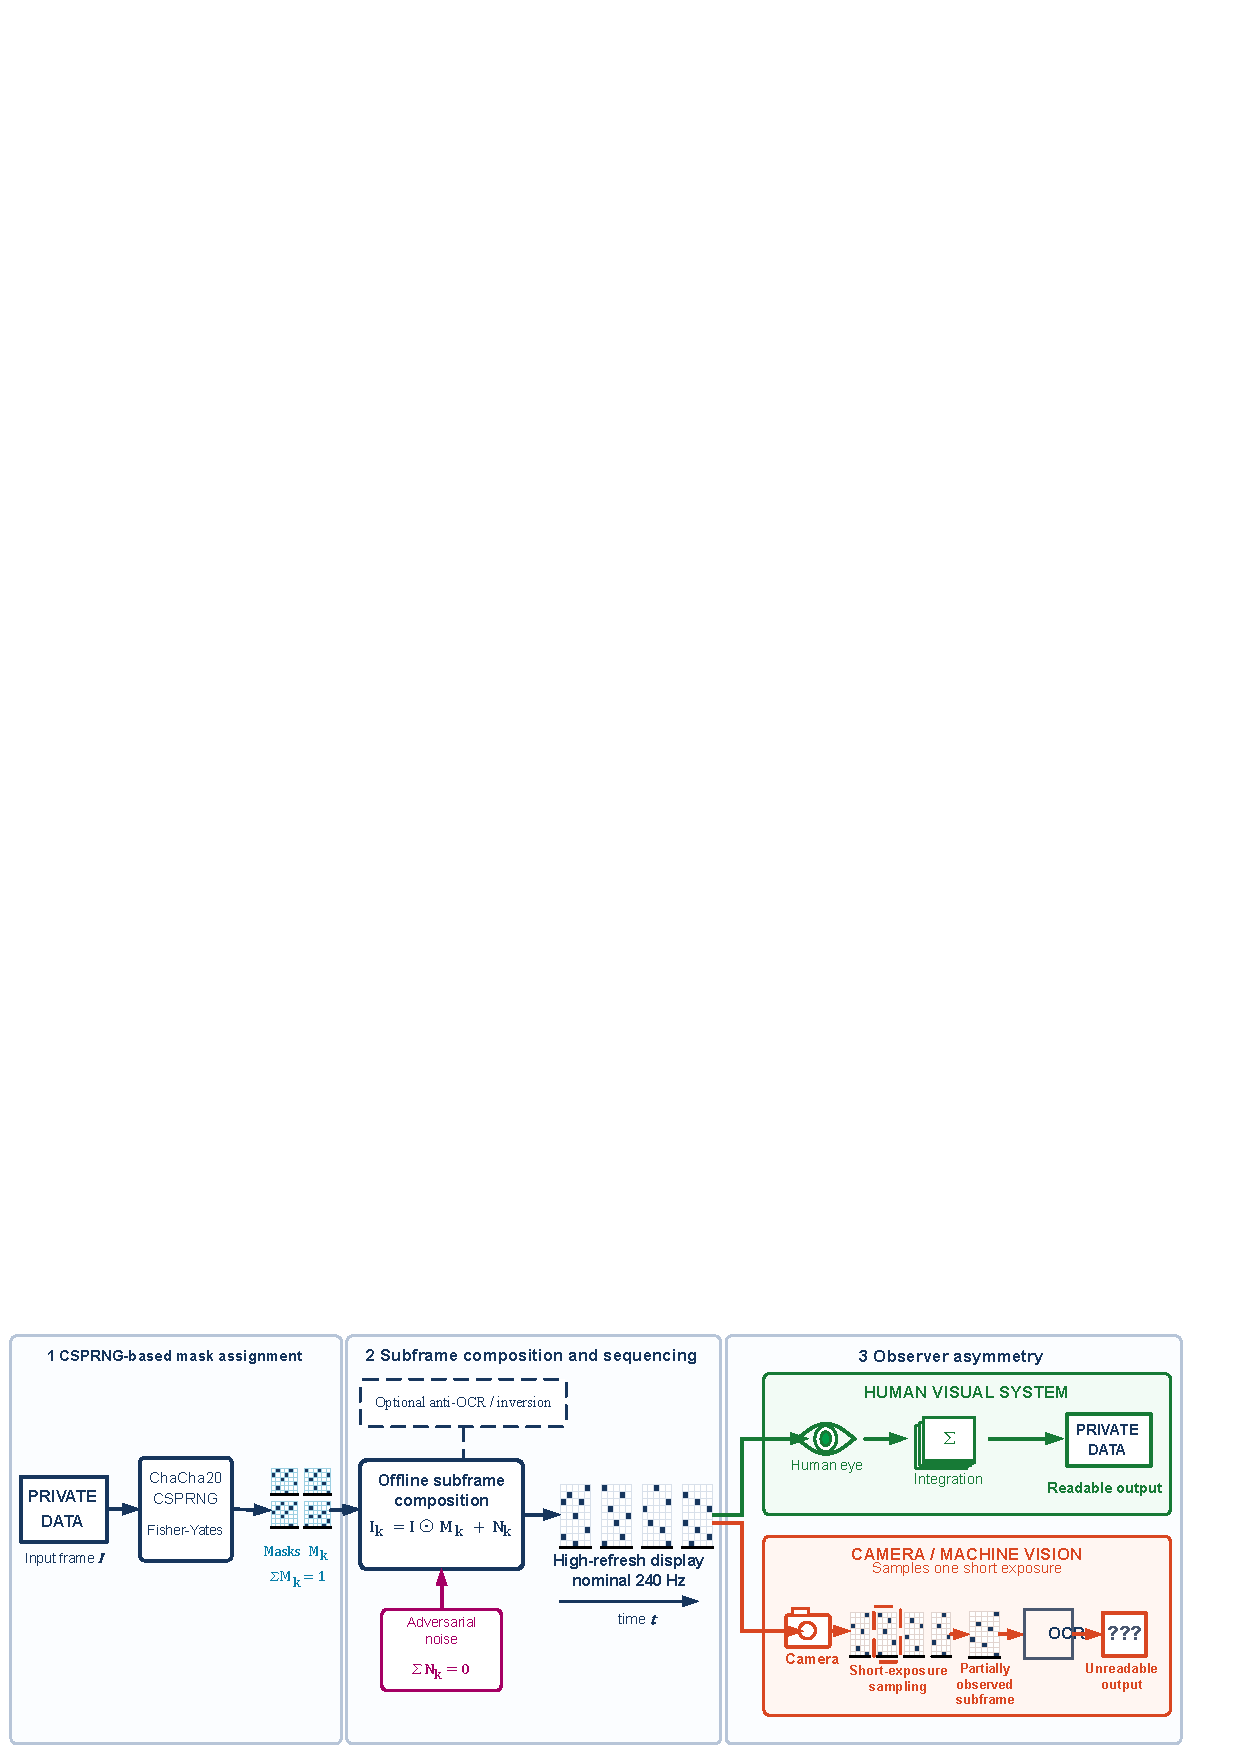
\includegraphics[width=\textwidth,viewport=0 0 515.52 206.16,clip]{figures/visio/figure2_method_pipeline/final/figure2_method_pipeline.pdf}
\caption{时域像素掩模系统管线：从原始内容到受保护显示。输入帧被分解为~CSPRNG~分配的互补像素掩模；在进行高刷播放前，插入可选的面向~OCR~的互补噪声、与配置档相关的条纹/字形覆盖层以及可选的部分反色帧。人类观察者预期能将多个时隙整合为可读视图，而短曝光相机可能仅捕获稀疏的子帧。长曝光和视频时域平均可累加多个时隙，因此作为边界攻击被单独评估，而非假定其不存在。}
\label{fig:pipeline}
\end{figure*}

\subsection{互补对抗噪声}

在子帧上叠加对抗噪声~$\mathbf{N}_1, \ldots, \mathbf{N}_n$，满足：
\begin{equation}
\sum_{k=1}^{n}\mathbf{N}_k = \mathbf{0}
\label{eq:noise_complement}
\end{equation}
式~(\ref{eq:noise_complement})~仅在叠加、裁剪和显示传递函数之前的理想线性域严格成立。已有工作表明微小文本图像扰动即可误导~OCR~系统~\cite{b_song2018}，为面向~OCR~的噪声设计提供了依据。噪声方向由~FGSM~\cite{b_goodfellow2015}~式代理梯度生成，幅度限制为~$\varepsilon=8/255$，再在时域中作互补分解。显示器不能输出负辐亮度，实现使用基底电平和数值裁剪，经~gamma、量化、裁剪和相机成像后噪声不保证物理上精确抵消。

\textbf{组件作用}：随机点阵掩模是主要机制。受控数字实验中噪声可抑制弱掩模或修复攻击下的残余结构，但真机短曝光结果显示~mask+noise（25.6\%）高于~mask-only（19.2\%），带微弱条纹/字形叠加的~Strong~档也略高于~mask-only（20.7\%~对~19.2\%）。对抗噪声和微弱幅度叠加并非跨所有物理条件的单调增强，而是可选的配置组件，收益取决于攻击方式、识别器和成像链路。

\subsection{亮度补偿}

每个像素在一个~$n$~时隙周期中仅点亮一次。理论上若显示器能在线性光域把点亮时隙的光输出提升~$n$~倍，周期平均亮度可接近原图，但当前~PoC~未实现逐时隙动态背光协同，也未用光度计验证绝对亮度。本文的亮度对齐、CIEDE2000~$\Delta E_{00}$~\cite{b_ciede2000}~和~SSIM~结果均来自数字积分/归一化模型，仅用于配置间对比，不作为面板光学等价或用户舒适度的证据。

\subsection{时序与带宽}

仅含~$n$~个互补子帧的基础周期，以~60\,Hz~为最低周期率，需~$f_r\geq60n$；$n=4$~时对应~240\,Hz。若额外包含一帧反色帧，条件变为~$f_r\geq60(n+1)$，240\,Hz~下周期率仅~48\,Hz，低于~60\,Hz~设计目标。FPI~是基于周期率和空间汇聚的模型化闪烁代理指标（数值越低预测闪烁风险越小），不是临床阈值。随机掩模的空间相位变化可能降低局部同步调制，但闪烁感知仍受亮度、对比度、视网膜位置和眼动影响~\cite{b_cai2024,b_davis2015}。

\subsection{抗拍强化档}
\label{sec:hardened}

基础线性时域掩模在完整周期时域平均攻击下会泄露（\S\ref{sec:security_frontier}），为此引入非线性增强档。除非另有说明，本节真机采集配置默认使用~$n=4$~基础时域掩模并启用互补对抗噪声。表~\ref{tab:real_ocr_main}~中”Mask + noise”行即为不含条纹/字形叠加的基础配置；Strong~档在此基础上加微弱条纹/字形，Deployed~档在~Strong~上加微弱反色帧，抗拍强化档则使用更强的条纹/字形设置和同样的微弱反色帧。
\begin{itemize}
\item \textbf{Strong（反~OCR）档}：在基础的掩模+噪声上，设置掩模单元大小为~1~像素，条纹宽度为~10~像素，条纹幅度~$\alpha_s=0.10$，字形幅度~$\alpha_g=0.12$，不含反色帧。

\item \textbf{Deployed~档}：在~Strong~档基础上加入~$\alpha=0.2$~的反色帧，作为可读优先的配置档。

\item \textbf{抗拍强化档（capture-hardened）}：在基础的掩模+噪声上，将掩模单元大小增至~2~像素，条纹宽度设为~6~像素，条纹和字形幅度分别增至~0.42~和~0.55，并加入~$\alpha=0.2$~的反色帧。
\end{itemize}

非线性档偏离严格完备性（$\sum\mathbf{I}_k \neq \mathbf{I}$），画面出现可感知的条纹和颗粒。这与~Kaleido~类时域重编码形成对照：后者依赖周期内人眼完备混合保障观看体验，完整周期积分能混合回近似原始画面，与其防盗录目标不冲突。本文面对的静态内容抓拍威胁中，完备性恰是积分攻击的入口，强化档以可见条纹和颗粒为代价换取对完整周期积分的鲁棒性。安全收益与可读性代价需分别报告；用户研究完成前不预设这种代价对所有场景都可接受。

\subsection{部分反色帧}

长曝光攻击指曝光窗口覆盖一个完整显示周期（$n=4$、240\,Hz~时基础周期约~16.7\,ms，含反色帧约~20.8\,ms；\S\ref{sec:setup}~实测使用~31.25~与~125\,ms），可通过传感器积分近似还原原始画面。缓解思路是在每~$n$~帧子帧周期后插入一帧\textbf{部分反色帧}~$\alpha \cdot (255 - \mathbf{I})$，使长曝光积分中叠入与原图互补的亮度分量以降低净信号对比度。$\alpha$~越大长曝光恢复可能越低，但数字积分视图的亮度和对比度也随之改变。

真机反色强度消融（表~\ref{tab:inversion_ablation}，管线同~\S\ref{sec:real_capture}）表明弱反色并未改善长曝光字符恢复：$\alpha=0$~为~68.6\%，$\alpha=0.2$~为~67.0\%（best-of-engine），$\alpha\in[0,0.5]$~各档的~95\%~置信区间大幅重叠。该消融固定~Strong~叠加层（$\alpha_s=0.10$，$\alpha_g=0.12$），仅变反色强度，使用~5~项内容子集（账号、代码、CET6）而非主配置的~12~项语料，$\alpha=0.2$~时的长曝光值（$N=135$）与表~\ref{tab:real_ocr_main}~Deployed~行~60.9\%（$N=324$）不是同一估计。只有接近全反色（$\alpha=1.0$）时才降至~18.1\%，但数字积分视图已严重退化。视频时域平均下弱反色档同样维持~64--73\%~字符恢复率。弱反色帧不能独立抵御积分类攻击；deployed~档取~$\alpha=0.2$~是模型化可读性优先的设计选择，非经用户研究验证的最优点。

\begin{table}[!t]
\caption{基于固定~Strong~叠加层（$\alpha_s=0.10$，$\alpha_g=0.12$）的反色帧强度~$\alpha$~消融：真机~best-of-engine~字符恢复率（均值与~95\%~Bootstrap CI，汇总~9~个几何条件下的~5~项账号/代码/CET6~子集；长曝光每档~$N=135$，视频时域平均每档~$N=45$）。这~5~项子集与表~\ref{tab:real_ocr_main}~中~Deployed~行的~12~项测试内容不同。}
\label{tab:inversion_ablation}
\centering
\small
\begin{tabular}{lcc}
\toprule
$\alpha$ & 长曝光~char~(\%) & 视频时域平均~char~(\%) \\
\midrule
0.0 & 68.6~[63.1, 73.9] & 72.7~[63.3, 81.1] \\
0.2 & 67.0~[61.3, 72.7] & 69.8~[59.9, 78.7] \\
0.3 & 72.0~[66.2, 76.9] & 64.3~[54.0, 73.6] \\
0.5 & 61.7~[55.6, 67.7] & 66.4~[56.5, 75.2] \\
1.0 & 18.1~[14.0, 22.0] & 28.4~[20.5, 36.9] \\
\bottomrule
\end{tabular}
\end{table}

每个显示周期由此包含~$n+1$~个时隙。$n=4$、240\,Hz~时周期率为~48\,Hz，低于本文设定的~60\,Hz~设计目标，可能产生可感知闪烁，且不存在适用于所有观察条件的固定“无闪烁阈值”。

\subsection{实现范围}

当前~PoC~位于应用/算法层，使用~Python~和~GPU~渲染生成显示序列，不含~OS~驱动级注入（DXGI / KMS-DRM / CoreDisplay），也不含逐时隙动态背光控制。本文验证的是显示序列及其拍摄结果，不等同于生产级系统集成。


%% ============================================================
%% V. 实验评估
%% ============================================================
\section{实验评估}
\label{sec:evaluation}

% 叙事逻辑：真机拍摄 OCR（5.2）→ 真机 VLM 探针（5.3）→ 用户体验（5.4）→ 检测/跟踪（5.5）→ 软件模拟补充（5.6）

\subsection{实验设置}
\label{sec:setup}

\textbf{硬件平台}：实验在一台配备~Intel Core i7-8700K（3.70\,GHz）、32\,GB RAM、NVIDIA TITAN Xp（12\,GB VRAM）的桌面工作站上运行。显示画布分辨率为~$1920 \times 1080$，显示器标称刷新率为~240\,Hz。该刷新率仅满足~$n=4$~基础子帧循环的~$f_r/n=60$\,Hz；若每周期插入一帧反色帧，周期频率为~$240/(n+1)=48$\,Hz，反色配置的舒适性不能由”240\,Hz~高刷”直接推出。

\textbf{拍摄设备}：物理拍摄实验定位为单一~UVC~摄像头可行性研究，使用~eMeet SmartCam S600~USB~网络相机（UVC~标准驱动）。回放画布为~$1920 \times 1080$，相机输出经透视校正和内容裁剪后再送入识别器。合并后的实验元数据显示，短曝光与视频帧曝光时间为~0.49~或~3.91\,ms，长曝光为~31.25~或~125\,ms，视频采集帧率为~60\,fps。摄像头分别放置在距显示器~0.5\,m、1\,m、1.5\,m~三个距离，每个距离下旋转~$0^{\circ}$、$15^{\circ}$、$30^{\circ}$~三个角度，共~9~组几何条件。该设置验证当前~UVC~链路可行性；环境照度未记录，未覆盖手机、智能眼镜或其他~ISP，结果不外推到这些设备。

\textbf{测试内容}：在~9~个几何位置的每一处，真机~OCR~采集实验使用了一组固定的~12~项测试内容：11~项选定的合成数据，以及~1~份~CET6（大学英语六级真题）文档（竖排~$900 \times 1280$）。每项内容采集~3~次，得到该位置下每种“配置档-攻击”条件下~36~张图像；结合~9~个位置，在考虑到已声明的~Deployed~档重复采集之前，共计~$12 \times 3 \times 9 = 324$~张图像。相比之下，软件模拟~OCR~实验使用了完整的~120~样本合成语料库（12~个内容模板~$\times$~10~变体，映射到涵盖密码、凭证、代码、表格、段落、URL~等的~9~个分类标签）。真机目标检测使用了包含~150~张图像的~COCO~val2017~\cite{b_coco2014}~子集；目标跟踪使用了~MOT17-09-FRCNN~\cite{b_mot16}~序列的~450~帧。模拟检测仅使用~8~张图像进行管线诊断；模拟跟踪覆盖了~5316~帧。真机短曝光~OCR~是主要可行性证据，检测/跟踪用于探索迁移风险，8~图模拟检测仅为管线诊断。

\textbf{评测指标}：OCR~字符恢复率定义为~$\max(0,1-\mathrm{CER})$。完全匹配率在移除空白并忽略大小写后判断全文是否一致。敏感~token~恢复率统计参考文本中数字、账号、URL/路径和密钥样式字段被完整找回的比例。泄露率是字符恢复率不低于~20\%~的样本比例。检测使用~mAP、mAP50~和~AR，跟踪使用~HOTA、IDF1，并在软件模拟中补充~MOTA/MOTP。对于未完成的用户调研，计划使用基于最小字符串距离的打字准确率/速度、首击延迟，以及可读性、闪烁感、即时视觉不适和感知隐私的五级~Likert~量表。

对于真机~OCR~主要结果，首先取每次拍摄中三个引擎的最大恢复率，以模拟攻击者选择最佳识别器的行为，然后以单次拍摄为重采样单元，使用固定的随机种子~20260612~进行~2000~次百分位数重采样，估计~95\%~Bootstrap~置信区间。核心条件的置信区间在~\S\ref{sec:real_capture}~中行内报告；消融区间见表~\ref{tab:inversion_ablation}。由于相同内容和几何条件下存在重复测量，这些区间描述的是当前语料库和采集设置下的经验不确定性，而非独立的总体推断。检测和跟踪结果未进行显著性测试；差异仅作描述性报告。

\textbf{数字可用性代理指标}：$\Delta E_{00}$~是原图与完整周期数字重建图之间的平均~CIEDE2000~色差；SSIM~是它们的平均结构相似度。归一化互信息代理定义为~$I(X;Y)/H(X)$，其中~$X$~为原始灰度图，$Y$~为单子帧灰度图，使用~64~个直方图~bin~估计；数值越低表示单子帧保留的信息越少。实现中的~FPI~使用简化模型：设单像素调制深度~$d=1-1/n$，空间汇聚像素数~$N=625$，像素照明频率~$f_p=f_r/n$。当~$f_p\geq60$\,Hz~时，$\mathrm{FPI}=dN^{-1/2}(60/f_p)^2$；低于~60\,Hz~时，公式使用~$d(1-f_p/60)$。注意该分段形式在~$f_p=60$\,Hz~处不连续：在略低于~60\,Hz~的窄带内，低频分支产生的值小于~60\,Hz~时的高频分支，这与“频率越低闪烁越严重”的直觉相悖。本文扫描的~12~个配置（$f_p$~网格点在~18--180\,Hz~之间）未落入该临界窄带，因此配置排序不受影响。该公式并非~IEEE~1789~标准指标或临床阈值；它仅用于本文内配置排序。

% ----------------------------------------------------------
\subsection{单一~UVC~摄像头真机拍摄~OCR~实验}
\label{sec:real_capture}

真机~OCR~实验语料共包含~10\,575~张图像，每个几何位置各~1\,175~张，全部来自同一款~eMeet SmartCam S600~UVC~网络相机。其中混合了组件消融、参数扫描和主攻击条件，因而不是“9~几何 $\times$ 7~档位 $\times$ 3~攻击”的平衡全因子设计。样本数的一处不对称需要说明：deployed~档在每个位置对~12~个拍摄内容条目中的~5~个（账号凭证~2、代码片段~2、CET6~文档~1）执行了两轮同参数采集，其余档位为一轮，故其短曝光/视频样本数为~459/153~而非~324/108，两轮样本均纳入统计。本文把总规模用于说明单~UVC~链路内的物理采集覆盖度，而把核心攻击条件子集作为主要可行性证据；这些结果不构成跨摄像头、跨手机或跨智能眼镜的统计验证。使用~Surya~\cite{b_surya2024}、EasyOCR~\cite{b_easyocr2020}、Tesseract~\cite{b_smith2007}~三个~OCR~引擎分别评测，共产生~31\,725~条引擎级记录。近年视觉语言模型已展现出较强~OCR~能力~\cite{b_shi2023}；\S\ref{sec:vlm}~的真机探针证实，传统~OCR~上的防护效果不能外推到~VLM~攻击者。表~\ref{tab:real_ocr_main}~报告核心条件子集，并对每次拍摄取~best-of-engine。表~\ref{tab:real_ocr_engine}~给出短曝光下的各引擎独立结果。图~\ref{fig:montage}~给出数字积分视图与短/长曝光实拍的定性对比，图~\ref{fig:bar_attack}~按档位~$\times$~攻击模式汇总恢复率。

\begin{table*}[!t]
\caption{单一~UVC~摄像头真机拍摄~OCR~核心条件结果（best-of-engine，$N$~为该行独立拍摄数，9~几何条件汇总）}
\label{tab:real_ocr_main}
\centering
\begin{tabular}{lllcccc}
\toprule
防护档位 & 攻击模式 & $N$ & Char~recovery & Exact~match & Sensitive~token & Leak~rate \\
\midrule
\multirow{3}{*}{original（未保护）}
 & short & 324 & 94.1\% & 65.7\% & 98.4\% & 99.4\% \\
 & video:temporal\_mean & 108 & 79.9\% & 61.1\% & 85.6\% & 86.1\% \\
 & long & 324 & 47.3\% & 18.8\% & 95.7\% & 58.6\% \\
\midrule
\multirow{3}{*}{mask\_only}
 & short & 324 & 19.2\% & 0.3\% & 30.8\% & 30.6\% \\
 & video:temporal\_mean & 108 & 79.0\% & 48.1\% & 84.0\% & 88.0\% \\
 & long & 324 & 67.2\% & 35.5\% & 94.0\% & 75.0\% \\
\midrule
\multirow{3}{*}{mask\_noise}
 & short & 324 & 25.6\% & 2.8\% & 34.4\% & 36.1\% \\
 & video:temporal\_mean & 108 & 79.2\% & 49.1\% & 83.9\% & 88.9\% \\
 & long & 324 & 68.0\% & 39.8\% & 95.7\% & 76.2\% \\
\midrule
\multirow{3}{*}{strong（anti\_ocr）}
 & short & 324 & 20.7\% & 0.6\% & 33.7\% & 32.4\% \\
 & video:temporal\_mean & 108 & 78.6\% & 50.9\% & 83.3\% & 88.9\% \\
 & long & 324 & 61.6\% & 39.8\% & 95.7\% & 71.3\% \\
\midrule
\multirow{3}{*}{deployed}
 & short & 459 & 15.1\% & 0.4\% & 24.0\% & 20.5\% \\
 & video:temporal\_mean & 153 & 71.1\% & 42.5\% & 78.5\% & 85.0\% \\
 & long & 324 & 60.9\% & 36.4\% & 96.5\% & 69.1\% \\
\midrule
\multirow{3}{*}{capture-hardened}
 & short & 324 & 5.0\% & 0.0\% & 6.5\% & 3.7\% \\
 & video:temporal\_mean & 108 & 47.9\% & 5.6\% & 45.6\% & 76.9\% \\
 & long & 324 & 9.3\% & 0.0\% & 34.9\% & 14.2\% \\
\bottomrule
\end{tabular}
\end{table*}

\textbf{核心发现}：

\begin{enumerate}
\item \textbf{短曝光恢复率下降}：未保护屏幕的短曝光~OCR~字符恢复率为~94.1\%（95\%~CI~[93.1, 95.0]；exact~65.7\%）。Strong~档（不含反色帧）为~20.7\%~char~/~0.6\%~exact；deployed~档（加~$\alpha=0.2$~反色帧）降至~15.1\%（CI~[13.3, 17.1]；exact~0.4\%），相对未保护降幅~83.9\%，达到~\S\ref{sec:threat}~的部署档目标。两档差值说明弱反色帧在当前设置下提供额外抑制，但~deployed~档包含额外重复采集（$N=459$~而非~324），5.6~百分点差值不作严格配对因果解释。抗拍强化档进一步降至~5.0\%（CI~[4.3, 5.8]；exact~0\%），exact-match~满足严格达标线，char~恢复率处~5\%~边缘且~CI~跨越阈值，不宣称完全满足。这些结果支持当前~eMeet S600~UVC~链路内的短曝光缓解可行性，不构成对其他相机、手机或智能眼镜的保证。

\item \textbf{积分类攻击是残余前沿}：长曝光与视频时域平均利用完整周期的线性互补性。Deployed~档在长曝光下仍恢复~60.9\%~char~/~36.4\%~exact（敏感~token~96.5\%），视频时域平均下~71.1\%~char~/~42.5\%~exact。但未保护长曝光基线仅~47.3\%~char，反而低于~deployed~的~60.9\%，说明固定相机参数对不同显示条件有非单调影响，这组绝对值不能解释为防护收益。弱反色帧（$\alpha=0.2$）不足以独立抵御时域积分；微弱~Strong~叠加层同样无效：mask-only~与~Strong~在视频时域平均下几乎相同（79.0\%~对~78.6\%），长曝光差异也小（67.2\%~对~61.6\%），bootstrap~CI~重叠。图~\ref{fig:tradeoff}~中单调的合成趋势在弱叠加幅度下并不产生可测量的真机积分恢复率下降；仅抗拍强化的幅度才带来实测下降，且泄露依然显著。主要有效性结论限定在单帧短曝光威胁模型，积分类攻击作为安全边界单列。

\item \textbf{抗拍强化档降低积分恢复率，代价尚未由用户实验量化}：长曝光~9.3\%~char（CI~[7.9, 10.9]）/~0\%~exact，视频时域平均~47.9\%~char（CI~[41.8, 54.0]）/~5.6\%~exact（CI~[1.9, 10.2]）。视频条件泄露明显，不应解读为攻击已闭合。47.9\%~是~9~位置合并值，位置间差异大：0.5\,m~三角度分别为~50.7\%/0\%/33.8\%，1.0\,m~为~61.1--69.4\%，1.5\,m~为~48.4--55.5\%。其中为~0~的位置（0.5\,m/$15^{\circ}$）是唯一采用~0.49\,ms~视频帧曝光校准的位置，视频帧明显欠曝；其余位置均为~3.91\,ms~校准，恢复率在~33.8--69.4\%~间非单调变化。合并值既受曝光校准影响又不代表任一具体位置的风险，部署评估应按最不利条件取值。数字积分~SSIM~显示安全性与重建失真的取舍（图~\ref{fig:tradeoff}），但非真机或人类主体证据。\S\ref{sec:user_study}~的用户调研仅覆盖~deployed~档打字任务与核心掩模消融，抗拍强化档的感知代价留待后续研究。

\item \textbf{几何条件趋势}：9~组条件（0.5--1.5\,m $\times$ 0--30$^{\circ}$）中，短曝光保护条件的恢复率总体低于对应未保护条件。设计不平衡且未建立推断模型，不据此主张距离或角度方向上存在统计意义的单调鲁棒性。
\end{enumerate}

\begin{figure}[!t]
\centering
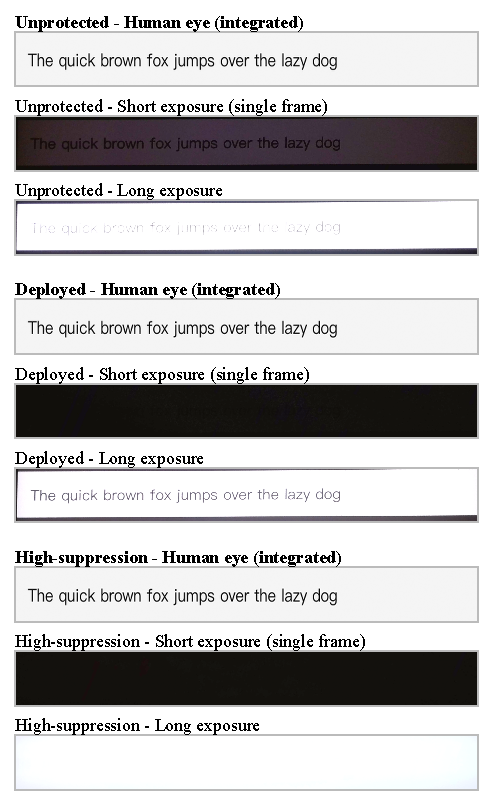
\includegraphics[width=\columnwidth]{figures/real_capture_montage.pdf}
\caption{真机拍摄蒙太奇：左列为数字积分重建视图，用于检查完整周期的图像一致性，中列为短曝光拍摄，右列为长曝光拍摄。数字积分视图不是人眼可读性或视觉舒适性的直接证据。}
\label{fig:montage}
\end{figure}

\begin{figure}[!t]
\centering
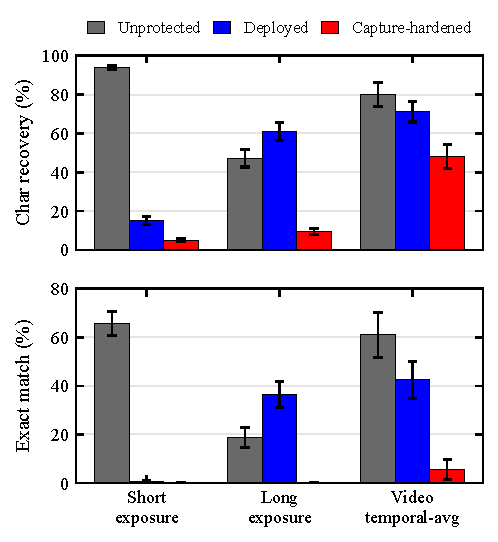
\includegraphics[width=\columnwidth]{figures/real_capture_bar.pdf}
\caption{真机防护效果：档位 $\times$ 攻击模式的~OCR~恢复率}
\label{fig:bar_attack}
\end{figure}

\begin{figure}[!t]
\centering
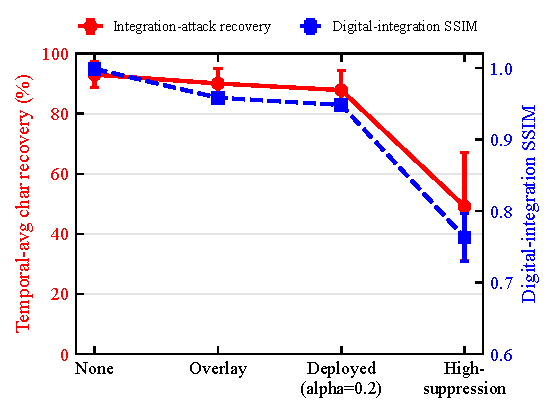
\includegraphics[width=\columnwidth]{figures/readability_robustness_tradeoff.pdf}
\caption{数字重建质量与积分攻击鲁棒性的取舍：随抗~OCR~叠加增强（无叠加~$\to$~strong~叠加~$\to$~deployed（叠加加~$\alpha=0.2$~反色帧）~$\to$~抗拍强化），时域平均字符恢复率下降（左轴），完整周期数字重建的~SSIM~\cite{b_wang2004}~也下降（右轴）。数据来自合成语料上的抗~OCR~档位消融（数字管线，非真机拍摄）；SSIM~是图像代理，不等同于用户可读性。}
\label{fig:tradeoff}
\end{figure}

\textbf{引擎间结果}：表~\ref{tab:real_ocr_engine}~按引擎拆分短曝光结果，图~\ref{fig:real_engine_ocr}~可视化所有六档。三引擎未保护条件下差异较大（Surya~37.1\%、EasyOCR~79.5\%、Tesseract~84.3\%）；deployed~档下各引擎为~3.2--11.7\%，抗拍强化档为~1.8--2.0\%。三种引擎均出现恢复率下降，但样本和引擎家族有限，不能据此声称与任意识别器无关。主表的~best-of-engine~按每次拍摄取三引擎最大值以模拟攻击者自由选择最佳识别器，数值不低于任一单引擎均值——这是对防守方更保守的报告口径。

\begin{table}[!t]
\caption{真机短曝光~OCR：三引擎分别结果（9~几何条件汇总）}
\label{tab:real_ocr_engine}
\centering
\small
\begin{tabular}{llccc}
\toprule
防护档位 & 引擎 & Char~(\%) & Exact~(\%) & N \\
\midrule
\multirow{3}{*}{original}
 & Surya & 37.1 & 22.8 & 324 \\
 & EasyOCR & 79.5 & 27.8 & 324 \\
 & Tesseract & 84.3 & 47.8 & 324 \\
\midrule
\multirow{3}{*}{mask\_only}
 & Surya & 4.2 & 0.3 & 324 \\
 & EasyOCR & 15.6 & 0.0 & 324 \\
 & Tesseract & 3.2 & 0.0 & 324 \\
\midrule
\multirow{3}{*}{mask\_noise}
 & Surya & 11.0 & 2.8 & 324 \\
 & EasyOCR & 18.1 & 0.0 & 324 \\
 & Tesseract & 4.8 & 0.0 & 324 \\
\midrule
\multirow{3}{*}{deployed}
 & Surya & 3.2 & 0.4 & 459 \\
 & EasyOCR & 11.7 & 0.0 & 459 \\
 & Tesseract & 3.3 & 0.0 & 459 \\
\midrule
\multirow{3}{*}{capture-hardened}
 & Surya & 1.8 & 0.0 & 324 \\
 & EasyOCR & 2.0 & 0.0 & 324 \\
 & Tesseract & 1.9 & 0.0 & 324 \\
\bottomrule
\end{tabular}
\end{table}

\begin{figure}[!t]
\centering
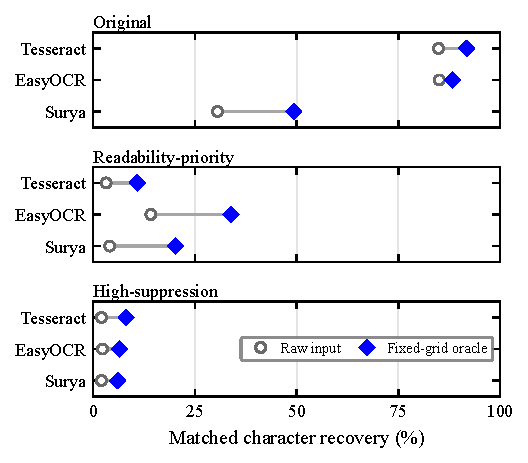
\includegraphics[width=\columnwidth]{figures/real_engine_ocr.pdf}
\caption{真机短曝光下三个~OCR~引擎在表~\ref{tab:real_ocr_engine}~中所有六个配置档位的字符恢复率，误差棒为以拍摄样本进行重采样的~95\%~Bootstrap~区间。三个引擎均受到抑制，但由于引擎家族有限，不能据此声称与任意识别器无关。}
\label{fig:real_engine_ocr}
\end{figure}

\subsection{真机拍摄~VLM~探针}
\label{sec:vlm}

为检验传统~OCR~结论能否外推到更强的端到端识别器，我们用三个商用视觉语言模型（Qwen3-VL-32B-Instruct、Kimi-K2.6、GLM-4.5V，经~SiliconFlow~API）识别同批真机照片。本节定位为\emph{边界/反例探针}：若~VLM~在传统~OCR~失败的图像上仍能恢复文本，则应用价值须限定在传统~OCR~短曝光缓解，不能宣称对现代~VLM~有效。

探针覆盖同一~UVC~摄像头的~0$^{\circ}$~轴向距离。近距离~0.5\,m~运行包含~156~张输入图像/聚合视图：同会话未保护短曝光基线~36~张、抗拍强化档短/长曝光各~36~张，以及由~60\,fps~录像离线合成的四种聚合视图各~12~段。新增~1.0\,m~和~1.5\,m~运行各包含抗拍强化档~120~张输入图像/聚合视图：短/长曝光各~36~张，四种视频聚合视图各~12~段。三个距离的~VLM~输入与表~\ref{tab:real_vlm}~的~OCR~BoE~参照列均为同批文件（短曝光/视频帧曝光~3.91\,ms、长曝光~31.25\,ms），参照值按~\S\ref{sec:setup}~的~best-of-engine~口径在同批文件上计算。输入均为原始相机~JPEG，不做对比度增强，与~OCR~管线对齐；试点中发现~CLAHE~类局部增强会部分重建被掩文字，相当于把预处理变成额外攻击组件。三次运行对应~1188~次模型请求，其中~1133~次得到可解析返回：0.5\,m~运行~468~次调用中~34~次失败（Qwen~2、Kimi~0、GLM~32），1.0\,m~运行~360~次中~21~次失败（Qwen~4、Kimi~1、GLM~16），1.5\,m~运行~360~次全部成功；各单元格均以有效调用数~$N$~报告。据此，本文把无失败的~1.5\,m~运行作为新增距离的主要完整证据，存在失败的~1.0\,m~运行仅纳入表~\ref{tab:real_vlm}~的短曝光距离扫描作描述性补充。1.0\,m~下，Qwen~与~Kimi~的长曝光~exact~分别为~84.4\%~和~74.3\%，三个模型的视频时域平均~exact~为~70.0--83.3\%，这些高恢复趋势与~1.5\,m~一致；但~GLM~长曝光~exact~仅为~3.3\%，明显低于~1.5\,m~的~58.3\%，因此不对三个模型作跨距离一致性概括，逐条结果见数据存档。为简洁起见，表~\ref{tab:real_vlm}~仅报告~0.5\,m~下的时域平均视频聚合视图作为完整的积分视图代表；其余~0.5\,m~聚合视图（单帧最佳、最佳滑动窗口平均以及最大投影）保留在数据存档中。无失败的~1.5\,m~运行则报告了所有四种聚合视图，以展示对视图选择的敏感性。模型标识为~Qwen/Qwen3-VL-32B-Instruct、Pro/moonshotai/Kimi-K2.6、zai-org/GLM-4.5V；解码温度为~0，最大输出~4096~token。三个模型共用同一条转写提示词：仅转写可见文字、禁止猜测缺失字符；参考真值不进入提示词。完整提示词、调用参数与逐次模型输出（转写文本、自报置信度与备注）随代码和数据存档（见“数据与代码可用性”）。指标计算与~\S\ref{sec:setup}~一致，按拍摄级汇总。CET6~真题为公开文档，可能落入模型训练语料使其字符恢复率被记忆抬高，因此合成私有片段与~exact-match~是更干净的判别口径。

\textbf{0.5\,m~会话选择透明性}：归档另保留同位置的~\texttt{real\_capture\_vlm\_d0.5\_a0\_rerun.json}（文件名时间戳~012715）替代会话；其中抗拍强化档短曝光输入近乎全黑，三模型转写均为空，char/exact~均为~0\%。该会话作为欠曝诊断留档，但不进入表~\ref{tab:real_vlm}~或与主运行平均。正文采用~141107、3.91\,ms~会话，是因为它与~OCR~参照列使用同批文件，且曝光更充分、对攻击者更有利；选择原则是输入对齐与保守报告，而不是按恢复率高低择优。由于没有独立光度计数据，本文只把“欠曝”作为由近黑图像和空转写共同支持的会话级诊断，不把它解释为已确定的相机~ISP~因果结论。

\begin{table*}[!t]
\caption{真机~VLM~探针（0$^{\circ}$~轴向距离；除~original~short~基线行外均为抗拍强化档）。每个~VLM~单元格为~Exact~/~Char~/$N$（\%~/~\%~/有效调用数）；OCR~BoE~列为同批文件上的三引擎~best-of-engine~参照（Exact~/~Char，\%）。}
\label{tab:real_vlm}
\centering
\footnotesize
\setlength{\tabcolsep}{4.2pt}
\begin{tabular}{llcccc}
\toprule
距离 & 条件 & OCR~BoE & Qwen3-VL-32B & Kimi-K2.6 & GLM-4.5V \\
\midrule
\multicolumn{6}{l}{\textit{短曝光距离扫描}}\\
\midrule
0.5\,m & original~short & 58.3~/~92.4 & 83.3~/~94.5~/~36 & 83.3~/~95.6~/~36 & 73.1~/~92.0~/~26 \\
0.5\,m & short & 0.0~/~8.4 & 77.8~/~91.5~/~36 & 47.2~/~84.7~/~36 & 51.6~/~70.8~/~31 \\
1.0\,m & short & 0.0~/~3.6 & 55.6~/~79.1~/~36 & 38.9~/~68.6~/~36 & 27.3~/~47.0~/~33 \\
1.5\,m & short & 0.0~/~6.5 & 47.2~/~68.9~/~36 & 33.3~/~61.5~/~36 & 36.1~/~70.0~/~36 \\
\midrule
\multicolumn{6}{l}{\textit{关键攻击视图}}\\
\midrule
0.5\,m & long & 0.0~/~2.1 & 82.4~/~85.7~/~34 & 2.8~/~7.9~/~36 & 0.0~/~4.9~/~30 \\
0.5\,m & video:temporal\_mean & 8.3~/~50.7 & 83.3~/~94.0~/~12 & 83.3~/~95.5~/~12 & 87.5~/~91.8~/~8 \\
1.5\,m & long & 0.0~/~13.2 & 91.7~/~89.3~/~36 & 88.9~/~89.9~/~36 & 58.3~/~62.4~/~36 \\
1.5\,m & video:single\_best & 0.0~/~4.3 & 8.3~/~24.8~/~12 & 0.0~/~12.7~/~12 & 0.0~/~29.8~/~12 \\
1.5\,m & video:temporal\_mean & 0.0~/~48.4 & 66.7~/~90.3~/~12 & 66.7~/~90.3~/~12 & 58.3~/~88.5~/~12 \\
1.5\,m & video:max\_proj & 0.0~/~19.0 & 66.7~/~90.1~/~12 & 58.3~/~89.2~/~12 & 58.3~/~88.7~/~12 \\
\bottomrule
\end{tabular}
\end{table*}

\begin{table}[!t]
\caption{0.5\,m~强化档短曝光按内容类型的~VLM~字符恢复率。基线列为同会话未保护~original~short~上~Qwen~的结果（Kimi/GLM~相近）；GLM~个别调用失败，括号内为其实际~$N$。1.5\,m~复跑中~CET6~密集页在三模型下均为~0\%~char。}
\label{tab:vlm_content}
\centering
\footnotesize
\setlength{\tabcolsep}{3.5pt}
\begin{tabular}{lcccc}
\toprule
内容类型~($N$) & 基线~(\%) & Qwen~(\%) & Kimi~(\%) & GLM~(\%) \\
\midrule
CET6~整页密集文档~(3) & 64.4 & 18.5 & 5.6 & 0.4 \\
账号/卡片凭证~(6) & 97.6 & 97.6 & 88.3 & 77.1~(5) \\
代码片段~(6) & 89.8 & 94.9 & 95.8 & 88.9 \\
数字串~(6) & 100.0 & 100.0 & 98.6 & 50.0~(4) \\
混合内容~(6) & 100.0 & 100.0 & 92.5 & 98.2~(4) \\
段落~(6) & 100.0 & 99.8 & 81.7 & 66.5 \\
英文短句~(3) & 95.3 & 95.3 & 96.9 & 94.6 \\
\bottomrule
\end{tabular}
\end{table}

表~\ref{tab:real_vlm}~给出~VLM~探针的合并结果：短曝光行用于观察距离变化，长曝光与视频聚合行用于观察积分类攻击边界。表~\ref{tab:vlm_content}~按内容类型拆分~0.5\,m~强化档短曝光的字符恢复率。

\textbf{核心发现}：

\begin{enumerate}
\item \textbf{VLM~给出主张边界而非扩大主张}：0.5\,m~同批照片中，三引擎~best-of-engine~在强化档短曝光下仅~char~8.4\%、exact~0\%，而~Qwen3-VL~达~char~91.5\%、exact~77.8\%。1.5\,m~复跑中三模型短曝光~exact~33.3--47.2\%、char~61.5--70.0\%。即便提示词禁止猜测，VLM~仍从可见碎片恢复大量文本。结论是传统~OCR~主张不能外推到~VLM~攻击者。

\item \textbf{失效集中在大字号短片段}：0.5\,m~下 CET6~整页文档的~VLM~恢复率为~0.4--18.5\%（未保护~64.4\%），而凭证、代码、数字串等大字号类别为~50--100\%（表~\ref{tab:vlm_content}）。1.5\,m~复跑中 CET6~密集页三模型均为~0\%~char/exact，数字串和短句仍高恢复。这与掩模粒度一致：小字号笔画~1--2~像素，移除~$1-1/n$~后拓扑不可重建；大字号字形在稀疏碎片与条纹下仍保留全局轮廓，被鲁棒视觉编码和语言先验补全。传统~OCR~依赖二值化与字符分割，被条纹阻断；VLM~不经过该瓶颈。

\item \textbf{攻击能力因模型和成像条件而异}：0.5\,m~长曝光下~Qwen3-VL~仍恢复~82.4\%~exact，而~Kimi/GLM~不超过~2.8\%；1.5\,m~长曝光~exact~升至~58.3--91.7\%。VLM~读屏能力同时受模型版本、距离、曝光和内容影响，”防住当前~VLM”的结论会随模型更新而过期。

\item \textbf{视频时域平均仍是~VLM~残余前沿}：0.5\,m~时域平均下三模型~exact~83.3--87.5\%、char~$\geq$91.8\%；1.5\,m~时域平均~exact~58.3--66.7\%、char~88.5--90.3\%。而~1.5\,m~单帧最优视频视图只有~0--8.3\%~exact，同批传统~OCR~在时域平均视图上~exact~不超过~8.3\%（char~48.4--50.7\%）。对~VLM~攻击者而言完整周期积分（\S\ref{sec:security_frontier}）比挑选单个清晰帧更危险，且不一定需要精确配准或复杂后处理。
\end{enumerate}

综上，抗拍强化档的有效性须按内容与攻击者类型限定：对传统~OCR~管线与密集小字成立；对配备~VLM~的攻击者，大字号短片段（凭证、代码、数字串）的短曝光防护已不成立。这把应用定位从”阻止任意机器读屏”收窄为”降低传统~OCR~短曝光批量恢复”，VLM-aware~显示防护是后续研究问题（对策方向见~\S\ref{sec:vlm_defense}）。本节覆盖单一相机、0$^{\circ}$~轴向距离、单档位与三个商业~API~模型，视频条件每格仅~12~段，商业模型可能随时间更新，数字应作描述性边界探针解读。

% ----------------------------------------------------------
\subsection{用户体验调研}
\label{sec:user_study}

为验证受保护显示对可读性和视觉舒适度的影响，设计了一项~Web~端用户调研。

\textbf{实验设备与环境协议}：同~\S\ref{sec:setup}~的~240\,Hz~显示器。正式研究版把实测刷新率硬门槛设为~$\geq200$\,Hz，以保证固定~$n=4$~基础子帧周期率~$f_r/n\geq50$\,Hz；低于门槛时禁止开始，不静默降低~$n$。144--199\,Hz~自适应路径仅供显式标记的演示模式使用，相关会话默认不进入统计。实验员在每位被试开始前确认固定显示器亮度、关闭自动亮度/省电与可变刷新、统一浏览器全屏、关闭高负载后台程序，并维持约~60\,cm~观看距离。任何显示模式变化后均重新检测刷新率。

浏览器在每个试次的~\texttt{requestAnimationFrame}~循环内记录实际帧间隔；若相邻回调间隔超过按试次前实测刷新率计算的期望间隔~1.5~倍，则计为丢帧事件，并保存估计丢帧数、丢帧率、平均/最大帧间隔、观测刷新率、基础子帧周期率和含反色帧的完整周期率。该记录只能反映浏览器呈现节奏，不能替代面板扫描或光度测量。

\textbf{伦理与安全}：本调研为最小风险的人类被试实验；作者所在机构对此类非医学行为实验不设伦理审查委员会，故未申请正式伦理批准，实验按下述知情同意与安全规程设计，但目前尚未开展正式数据采集。实验开始前，被试须分别勾选知情同意和光敏性筛查：页面明确提示掩模显示包含快速时间调制，出现不适、眼疲劳、头晕、恶心或头痛应立即停止，被试可在任意时刻无条件退出；自报有光敏性癫痫病史或对闪烁敏感者不得进入实验。系统保存同意时间和筛查通过标记。实现层面设有~$f_r/n\geq50$\,Hz~安全门；240\,Hz~面板上~$n=4$~的基础周期率为~60\,Hz。反色帧使完整周期频率降为~$f_r/(n+1)=48$\,Hz，实现对此单独记录告警与实际时序：$\alpha=0.2$~为低调制深度的弱反色帧，但其舒适性仍由本用户研究而非设计假设判断。登记信息（学号、姓名）仅用于参与管理，分析与发布只使用去标识化数据；年龄与性别为可选人口学字段。

\textbf{任务设计}：每位被试先完成一次~12~秒、不计分的未遮罩~Canvas~打字热身，再观看一次~10~秒、不计分的~deployed~完整遮罩预览，使首次正式~masked~试次不再同时承担熟悉刺激的作用，随后完成四轮~20~秒计分试次（被试内设计）。两种条件各重复两次，并按实验员预先连续登记的零起始序号~$k$~采用~ABBA~或~BAAB~顺序以平衡练习与疲劳效应：（A）\textbf{原始文本}（control），以~$n=1$~的未遮罩~Canvas~显示；（B）\textbf{掩模文本}（masked），采用实际部署配置，即~$n=4$，mask+noise，strong~anti-OCR~档（$\alpha_s=0.10$，$\alpha_g=0.12$，6~周期）+~弱反色帧（$\alpha=0.2$）。具体地，打字顺序索引为~$k\bmod2$，主观评分的拉丁方行号为~$\lfloor k/2\rfloor\bmod6$；因此每连续~12~名被试完整覆盖~$2\times6$~种联合分配，从而保证联合顺序分配的确定性与均衡性。正式会话的~$k$~在数据库中具有唯一约束，后端会重新计算并核对两个顺序索引。两条件均由同一~\texttt{renderSourceCanvas}~路径生成深底亮字，画布尺寸、23\,px~粗体字号和颜色完全一致，唯一处理差异为时域保护管线，从而避免正负极性和字重混淆。此处“周期”指~Web~端实现中掩模、噪声与条纹图案在多少个不同实现间轮换后重复，取值~6~可避免长曝光拍摄将单一固定图案积分为可辨认残留，与~\S\ref{sec:method}~描述的真机采集配置共享~$\alpha_s$、$\alpha_g$~参数但为~Web~播放专属设置。

计分不再逐位置比较字符，而将完整转录串与最优目标前缀作~Levenshtein~最小字符串距离（MSD）对齐~\cite{b_soukoreff2003}；未输入的目标后缀不计错，据对齐结果计算~accuracy、CPM~和~WPM，并保存编辑距离、对齐前缀长度和计分版本。另记录从点击“开始”到第一个有效输入事件的首击延迟。分析时先对每位被试同条件的两次试次取均值，再进行被试内配对比较。

\textbf{主观评分}：打字试次后，被试对~6~种条件分别在~4~个维度上做~1--5~Likert~评分：可读性（readability）、闪烁感（flicker）、即时视觉不适（fatigue~字段）和感知隐私（privacy）。条件包括未遮罩原文锚点、$n\in\{2,3,4\}$~mask+noise、$n=4$~mask-only，以及与打字条件相同的~$n=4$~deployed~完整配置（mask+noise+strong anti-OCR+弱反色）。其中前三个掩模层数均能在~240\,Hz~面板上保持不低于~60\,Hz~的真实时域播放；原设计中的~$n=8$~会得到~30\,Hz~并触发静态回退，故不再作为时域消融。六条件采用六阶平衡拉丁方呈现；每个条件至少观看~10~秒后才启用提交，并保存观看起止时间与时长。未遮罩锚点兼作注意力/量表解释辅助，但不预先以“必须评分~5”作为机械排除规则。本调研不含抗拍强化档，其明显条纹与颗粒的可接受性评估仍留作后续工作（见~\S\ref{sec:discussion}）。

\textbf{样本量与分析计划}：计划至少招募~$N=24$，该数值位于预期配对效应量~$d_z\approx0.6$--$0.8$、80\%~功效所需范围内，并恰好覆盖两轮~12~人的联合顺序分配。开跑前固定排除标准：debug/demo~会话、未完成全部四条打字或六条评分记录、实测刷新率低于~200\,Hz、任一打字试次尝试输入少于~5~个字符、control~平均准确率低于~50\%、masked~试次非时域模式，或试次内观测基础周期率低于~50\,Hz。WPM、CPM、accuracy、尝试字符数和首击延迟对每位被试先取条件均值；速度指标必须与准确率联合解释，避免把低正确率下的快速输入误判为性能提升。配对差值通过预先指定的~Shapiro~检验时用配对~$t$~检验，否则用~Wilcoxon~符号秩检验，并报告效应量和被试级~bootstrap 95\%~置信区间。Likert~数据按维度使用~Friedman~检验和~Holm~校正的事后配对~Wilcoxon~检验。分析脚本直接从正式数据库~\texttt{study\_formal.db}~生成去标识化参与者均值、JSON~审计报告和两张~\LaTeX~表。

\textbf{被试}：\TODO{最终被试人数及人口统计。}

\TODO{表：打字试次客观指标（accuracy/CPM/WPM，control vs masked，配对差异 + CI）。}

\TODO{表：6~条件 $\times$ 4~维度的 Likert 均值 + 标准差。}

\TODO{核心结论：deployed~完整配置下打字准确率/速度与首击延迟是否有显著变化；主观可读性、闪烁感和即时视觉不适评分情况。}

% ----------------------------------------------------------
\subsection{真机拍摄目标检测与跟踪实验}
\label{sec:detection}

为考察文字以外的视觉任务是否受同类退化影响，本节报告一组探索性检测/跟踪压力测试，定位为同一~UVC~设置下的跨任务边界探索，证据强度不与~OCR~主实验等同。内容显示在~240\,Hz~屏上，eMeet~S600~在~1.5\,m~/~$0^{\circ}$~下采集，离线运行四个检测器~\cite{b_yolo26,b_rtdetr2024,b_fasterrcnn2015,b_retinanet2017}，以~real\_clean（未保护实拍）为参照（表~\ref{tab:real_coco}）。跟踪使用~MOT17-09-FRCNN~450~帧，采用逐源帧停帧拍摄流程而非连续视频同步（表~\ref{tab:real_mot}）。关联器是受~ByteTrack~\cite{b_bytetrack2022}~启发的贪心回退实现，非官方~ByteTrack。real\_clean~部分控制了链路退化，但曝光与受保护显示间可能存在交互，差异不能全部作单一因果归因。

\begin{table}[!t]
\caption{真机~COCO~检测（150~图，real\_clean~为未保护实拍基线）}
\label{tab:real_coco}
\centering
\small
\begin{tabular}{llccc}
\toprule
检测器 & 条件 & mAP & mAP50 & AR \\
\midrule
\multirow{3}{*}{YOLO26x}
 & real\_clean & 28.6\% & 43.9\% & 31.0\% \\
 & real\_short & 1.3\% & 2.4\% & 1.4\% \\
 & real\_video & 3.5\% & 5.3\% & 3.6\% \\
\midrule
\multirow{3}{*}{RT-DETR-x}
 & real\_clean & 30.1\% & 50.2\% & 34.8\% \\
 & real\_short & 3.5\% & 5.8\% & 4.1\% \\
 & real\_video & 4.6\% & 7.3\% & 5.5\% \\
\midrule
\multirow{3}{*}{Faster~R-CNN}
 & real\_clean & 21.3\% & 39.2\% & 28.7\% \\
 & real\_short & 0.8\% & 1.6\% & 0.9\% \\
 & real\_video & 1.5\% & 3.0\% & 1.8\% \\
\midrule
\multirow{3}{*}{RetinaNet}
 & real\_clean & 22.6\% & 39.4\% & 27.0\% \\
 & real\_short & 0.9\% & 1.8\% & 1.0\% \\
 & real\_video & 1.9\% & 3.1\% & 2.0\% \\
\bottomrule
\end{tabular}
\end{table}

\begin{table}[!t]
\caption{真机~MOT17-09-FRCNN~停帧采集跟踪（ByteTrack~风格贪心关联，450~帧）}
\label{tab:real_mot}
\centering
\begin{tabular}{llcc}
\toprule
检测器 & 条件 & HOTA & IDF1 \\
\midrule
\multirow{3}{*}{YOLO26x}
 & real\_clean & 15.8\% & 12.1\% \\
 & real\_short & 8.7\% & 6.5\% \\
 & real\_video & 10.0\% & 8.7\% \\
\midrule
\multirow{3}{*}{RT-DETR-x}
 & real\_clean & 14.2\% & 10.4\% \\
 & real\_short & 8.1\% & 5.2\% \\
 & real\_video & 9.6\% & 6.8\% \\
\midrule
\multirow{3}{*}{Faster~R-CNN}
 & real\_clean & 14.4\% & 9.6\% \\
 & real\_short & 6.8\% & 6.0\% \\
 & real\_video & 10.5\% & 7.1\% \\
\midrule
\multirow{3}{*}{RetinaNet}
 & real\_clean & 14.2\% & 9.8\% \\
 & real\_short & 5.1\% & 4.4\% \\
 & real\_video & 6.8\% & 5.9\% \\
\bottomrule
\end{tabular}
\end{table}

短曝光条件下四检测器~mAP50~由~39.2--50.2\%~降至~1.6--5.8\%（图~\ref{fig:real_det_drop}），相对下降均超~85\%。real\_video~为~3.0--7.3\%，同样低于~real\_clean~基线。单帧破坏不只影响字符分割式~OCR，但仅一个相机、一个位置和~150~张图，不外推为跨设备检测防护结论。停帧跟踪中~HOTA~由~14.2--15.8\%~降至~5.1--8.7\%，IDF1~由~9.6--12.1\%~降至~4.4--6.5\%。但~real\_clean~基线~HOTA~本身已被停帧链路压低至~14.2--15.8\%，远低于原生图像常见水平，压缩了可下降空间，跟踪结果仅提供方向性证据。停帧流程不能替代连续视频跟踪实验。

\begin{figure}[!t]
\centering
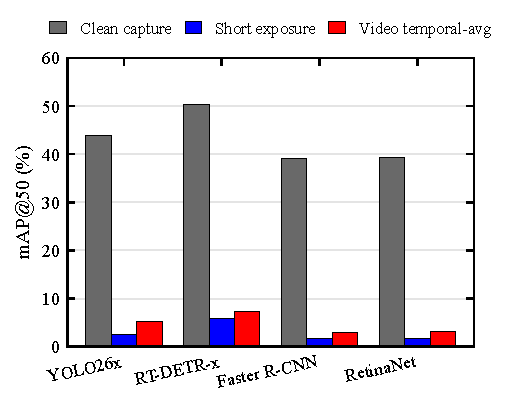
\includegraphics[width=\columnwidth]{figures/real_detection_drop.pdf}
\caption{真机检测：四个检测器~mAP50~在受保护条件下的跌幅}
\label{fig:real_det_drop}
\end{figure}

% ----------------------------------------------------------
\subsection{软件模拟补充实验}
\label{sec:simulation}

本节通过软件模拟补充两个问题：（1）攻击者只能获得单个受保护子帧时的机器可读性；（2）无相机噪声且精确对齐时的恢复边界。问题（1）同时刻画常规单帧截屏场景：截屏工具获取某一时刻的帧缓冲，对应单个受保护子帧，下文~0--2.6\%~的恢复率构成单帧截屏缓解证据。边界明确：恶意软件若在掩模前截获原始帧，或以录屏方式累加完整周期多帧，本方法不能保护。对截屏场景仅主张单帧层面缓解，不作”防截屏”保证。

\subsubsection{合成单子帧~OCR}
Tesseract~\cite{b_smith2007}、EasyOCR~\cite{b_easyocr2020}、Surya~\cite{b_surya2024}~在~120~条合成语料上的字符恢复率从~94.0--97.0\%~降至~0--2.6\%（表~\ref{tab:ocr_corpus}）。结果仅覆盖当前语料、参数和三个引擎，不足以证明对所有语言或识别器有效。

\begin{table}[!t]
\caption{合成单子帧：三引擎~OCR~字符恢复率（120~语料，$n=4$, $\varepsilon=8/255$）}
\label{tab:ocr_corpus}
\centering
\begin{tabular}{lccc}
\toprule
OCR~引擎 & 原始帧 & 单子帧 & 降幅 \\
\midrule
Tesseract & 94.0\% & 0.0\% & 94.0\% \\
EasyOCR & 94.1\% & 0.0\% & 94.1\% \\
Surya & 97.0\% & 2.6\% & 94.4\% \\
\bottomrule
\end{tabular}
\end{table}

\begin{figure}[!t]
\centering
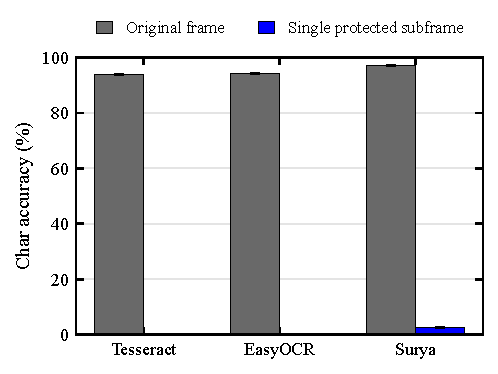
\includegraphics[width=\columnwidth]{figures/multiengine_ocr.pdf}
\caption{三个~OCR~引擎在原始帧和单个受保护子帧上的字符恢复率，误差棒为以语料样本重采样的~95\%~bootstrap~区间。}
\label{fig:multiengine_ocr}
\end{figure}

图~\ref{fig:multiengine_ocr}~将表~\ref{tab:ocr_corpus}~的三引擎结果可视化。三者在当前数据上的单子帧字符恢复率均不高于~2.6\%，表明结果不是由其中某一个引擎单独造成。更广泛的识别器泛化仍需额外实验。

\subsubsection{理论安全边界}
\label{sec:security_frontier}
攻击者在理想条件下叠加~$\geq n$~帧覆盖完整周期时，互补性被精确利用，对抗噪声（式~(\ref{eq:noise_complement})）同时被抵消，恢复率升至~95.2\%（逐样本最强攻击）——这是线性时域方案的\emph{原理性边界}。抗拍强化档在真机积分条件下降低了恢复率，但视频平均仍~47.9\%，只能称为缓解而非闭合。

\subsubsection{与软件代理基线对比}
9~个分层样本的探索性模拟中，调暗、高斯模糊、像素化、离轴隐私膜代理和单时域掩模子帧的字符恢复率分别为~92.9\%、52.6\%、0\%、84.7\%~和~0\%。调暗~50\%~与未保护条件同为~92.9\%，该参数未降低~OCR~恢复率。各处理的参数、物理条件和体验并未等价匹配（”隐私膜”只是软件离轴代理），图~\ref{fig:baselines_scatter}~仅展示当前代理设置下的权衡。

\begin{figure}[!t]
\centering
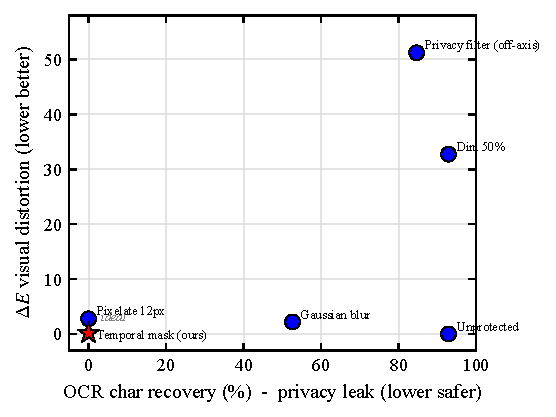
\includegraphics[width=\columnwidth]{figures/baselines_scatter.pdf}
\caption{9~个样本上的软件代理基线：横轴为~OCR~字符恢复率，纵轴为数字重建视图的~$\Delta E_{00}$。各方法参数和物理条件并未等价匹配，图仅作探索性比较。}
\label{fig:baselines_scatter}
\end{figure}

\begin{figure*}[!t]
\centering
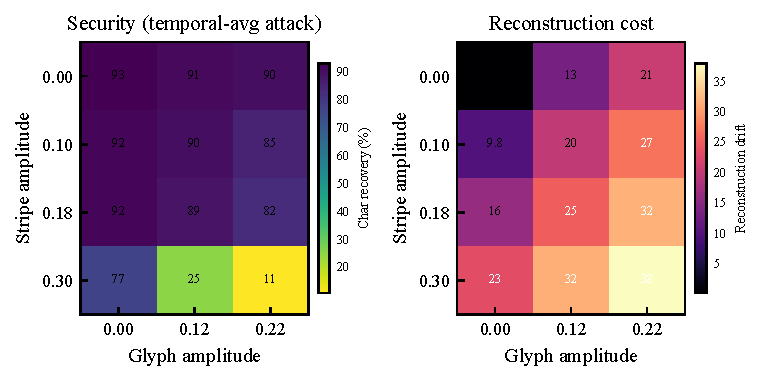
\includegraphics[width=0.82\textwidth]{figures/antiocr_heatmap.pdf}
\caption{抗~OCR~档位的条纹~$\times$~字形幅度网格（时域平均攻击）：左为字符恢复率，右为数字重建漂移。高条纹和高字形幅度区域的字符恢复率在当前~12~个参数格点（每格点~16~个样本）中描述性地降至~$\sim$11\%，同时重建代价上升。未进行显著性检验。}
\label{fig:antiocr_heatmap}
\end{figure*}

抗~OCR~档位的条纹/字形参数取舍见图~\ref{fig:antiocr_heatmap}。

\subsubsection{检测与跟踪模拟评测}
在~COCO~val2017~\cite{b_coco2014}和~MOT17~\cite{b_mot16}~上运行补充模拟。四个检测器为~YOLO26x~\cite{b_yolo26}、RT-DETR-x~\cite{b_rtdetr2024}、Faster R-CNN~\cite{b_fasterrcnn2015}~和~RetinaNet~\cite{b_retinanet2017}。COCO~模拟只有~8~张图，定位为实现管线诊断（表~\ref{tab:coco_sim}）。MOT~模拟覆盖~7~条序列共~5316~帧，使用受~ByteTrack~\cite{b_bytetrack2022}~启发的贪心关联回退实现（表~\ref{tab:mot_sim}）。由于~TrackEval~运行失败，表中~MOTA/MOTP/IDF1~来自项目内近似评测后端，不等同于官方~ByteTrack/TrackEval~结果。

\begin{table}[!t]
\caption{COCO~val2017~模拟检测管线诊断（4~检测器，8~张，不作数据集级性能估计）}
\label{tab:coco_sim}
\centering
\small
\begin{tabular}{llccc}
\toprule
检测器 & 条件 & mAP & mAP50 & AR \\
\midrule
\multirow{3}{*}{YOLO26x}
 & clean & 48.1\% & 58.3\% & 51.0\% \\
 & 单子帧 & 0.0\% & 0.0\% & 0.0\% \\
 & 时域平均 & 14.3\% & 18.3\% & 14.3\% \\
\midrule
\multirow{3}{*}{RT-DETR-x}
 & clean & 47.1\% & 58.7\% & 53.4\% \\
 & 单子帧 & 5.2\% & 6.0\% & 5.2\% \\
 & 时域平均 & 16.8\% & 23.7\% & 17.9\% \\
\midrule
\multirow{3}{*}{Faster R-CNN}
 & clean & 38.2\% & 52.7\% & 43.6\% \\
 & 单子帧 & 3.0\% & 4.4\% & 3.0\% \\
 & 时域平均 & 11.1\% & 16.5\% & 11.1\% \\
\midrule
\multirow{3}{*}{RetinaNet}
 & clean & 33.2\% & 47.1\% & 35.3\% \\
 & 单子帧 & 3.3\% & 4.2\% & 3.3\% \\
 & 时域平均 & 9.6\% & 13.2\% & 9.6\% \\
\bottomrule
\end{tabular}
\end{table}

\begin{table}[!t]
\caption{MOT17~模拟跟踪（ByteTrack~风格贪心关联，项目内近似指标，5316~帧）}
\label{tab:mot_sim}
\centering
\begin{tabular}{llccc}
\toprule
检测器 & 条件 & MOTA & MOTP & IDF1 \\
\midrule
\multirow{3}{*}{YOLO26x}
 & clean & 31.1\% & 81.7\% & 27.1\% \\
 & 单子帧 & 0.1\% & 74.8\% & 0.1\% \\
 & 时域平均 & 9.1\% & 78.1\% & 12.0\% \\
\midrule
\multirow{3}{*}{RT-DETR-x}
 & clean & 24.1\% & 79.8\% & 38.2\% \\
 & 单子帧 & $-$2.3\% & 73.2\% & 5.4\% \\
 & 时域平均 & $-$11.4\% & 75.0\% & 14.7\% \\
\midrule
\multirow{3}{*}{Faster~R-CNN}
 & clean & 3.8\% & 77.9\% & 35.6\% \\
 & 单子帧 & $-$2.5\% & 71.2\% & 4.5\% \\
 & 时域平均 & $-$2.7\% & 73.2\% & 14.0\% \\
\midrule
\multirow{3}{*}{RetinaNet}
 & clean & $-$5.4\% & 77.1\% & 30.5\% \\
 & 单子帧 & 0.4\% & 70.6\% & 2.7\% \\
 & 时域平均 & $-$2.9\% & 73.8\% & 11.9\% \\
\bottomrule
\end{tabular}
\end{table}

8~张图上单子帧~mAP50~为~0--6.0\%，样本量仅足以检查趋势。5316~帧近似跟踪中单子帧~IDF1~0.1--5.4\%，MOTA~存在负值和非单调现象。图~\ref{fig:all_attackers}~汇总当前评测中单子帧相对~clean~基线的剩余能力。

\begin{figure}[!t]
\centering
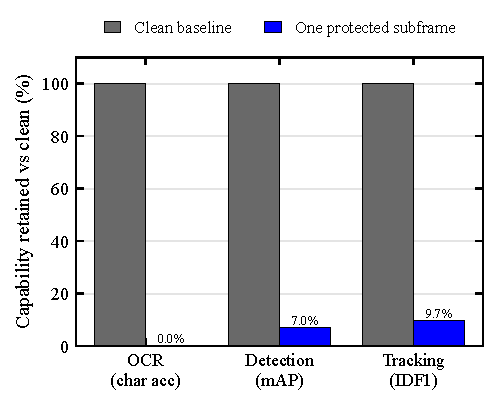
\includegraphics[width=\columnwidth]{figures/all_attackers.pdf}
\caption{当前评测中单个受保护子帧的相对剩余能力（clean~=~100\%），OCR、检测和跟踪约为~0--9.7\%。该图仅汇总所测模型与指标。}
\label{fig:all_attackers}
\end{figure}

\subsubsection{安全--可用性权衡}
模型扫描覆盖~$n\in\{2,4,6,8\}$~与刷新率~$\in\{144,240,360\}$\,Hz~共~12~个组合，Pareto~前沿基于~(FPI, 归一化互信息)~双目标最小化。选择规则：先保留~$\mathrm{FPI}<0.1$~的安全候选（超阈值即排除，如~$n=8$~@~360\,Hz~的~FPI\,=\,0.219），再在安全候选中取归一化互信息最小者。选出~$n=6$~@~360\,Hz（FPI\,=\,0.033，归一化互信息~$=0.249$，$\Delta E_{00}=0.60$，SSIM\,=\,0.9995）。基础配置~$n=4$~@~240\,Hz~归一化互信息为~$0.377$，高于~$n=6$~候选——后者以更高~$\Delta E_{00}$（0.60~对~0.34）换取更低的单子帧信息保留。这只是数字模型筛出的候选，未在~360\,Hz~实体显示器或用户研究中验证，非部署推荐。图~\ref{fig:pareto}~展示各组合下的~Pareto~前沿。

\begin{figure}[!t]
\centering
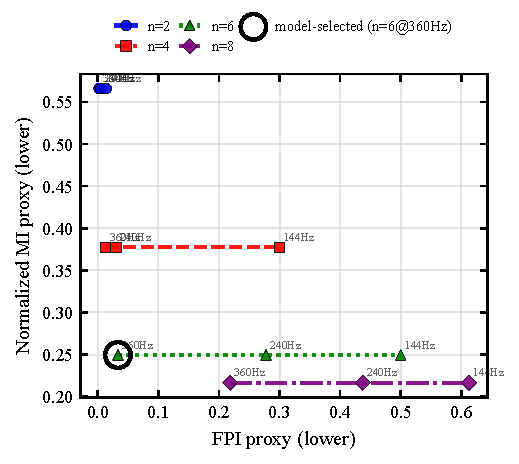
\includegraphics[width=\columnwidth]{figures/pareto_sweep.pdf}
\caption{数字模型中的安全--可用性代理~Pareto~前沿：$n \times$~刷新率，FPI~与归一化互信息均非用户体验或真实攻击成功率的直接测量。}
\label{fig:pareto}
\end{figure}


%% ============================================================
%% VI. 讨论
%% ============================================================
\section{讨论}
\label{sec:discussion}

\subsection{证据层级与主张范围}

本文最直接支持的结论：在当前~eMeet S600~单~UVC~摄像头、显示器、语料和~9~组几何条件下，时域像素掩模大幅降低了传统~OCR~攻击者在短曝光屏幕照片中的字符恢复和全文匹配。10\,575~张图像反映该~UVC~链路内的组件与攻击条件覆盖度，非平衡全因子设计，只覆盖一款网络相机，不构成跨设备或跨场景统计推断。检测/跟踪、VLM~探针和软件模拟分别回答退化迁移性、更强识别器突破能力和完整周期积分边界，共同划定边界而非扩大有效性主张。

\subsection{线性积分的数学张力}

本方案利用人眼积分与相机单帧采样之间的差异，但人眼积分本质是线性求和（$\sum\mathbf{I}_k = \mathbf{I}$），相机做同样的多帧累加也能还原原始信息——这是所有基于视觉暂留的时域方案共有的原理性边界。VLM~对抗鲁棒性研究~\cite{b_li2025}~表明大模型在受扰图像上仍可提取部分语义，\S\ref{sec:vlm}~的真机探针证实了该风险：VLM~从单张短曝光照片即可恢复大字号内容，从时域平均和长曝光视图中获得更强信号。\S\ref{sec:security_frontier}~量化了积分边界：完整周期积分可恢复~95.2\%。

\subsection{抗拍强化档的作用与代价}

抗拍强化档以条纹和字形扰动打破严格完备性，使当前积分条件下恢复率下降，但数字重建指标同时变差。\S\ref{sec:real_capture}~中该档短曝光~exact-match~0\%，视频时域平均~exact-match~5.6\%，字符恢复率仍~47.9\%，只能视为缓解而非完全阻断。条纹和颗粒是否可被用户接受须由用户实验回答，\S\ref{sec:user_study}~的设计仅覆盖~deployed~档与核心掩模条件，该档可接受性仍是未回答的问题。

\subsection{VLM~攻击者与对策方向}
\label{sec:vlm_defense}

\S\ref{sec:vlm}~显示防护失效集中于大字号短片段，时域平均/长曝光进一步放大~VLM~可利用的信号。本文将该结果作为主要边界贡献保留在正文——它直接决定方法的可部署叙事：当前方案可作为传统~OCR~短曝光缓解，不能作为现代~VLM~读屏防护。对症方向：（1）\textbf{字号自适应掩模粒度}，令~mask~cell~随渲染笔画宽度缩放，使单子帧不再保留字符拓扑；（2）\textbf{互补字形诱饵}，在~$\sum_{k}\mathbf{N}_k=\mathbf{0}$~框架内注入周期内互消的假笔画与假字符，使单帧攻击者得到高置信错误文本而非部分正确文本；（3）\textbf{部署层内容策略}，将凭证等高危字段以密集小字渲染或按字段启用强化档。以上方向均未经实验验证。针对~VLM~视觉编码器的对抗扰动受数字到物理迁移性限制（\S\ref{sec:related}），预期收益有限。更一般地，观察者在积分窗口内可见的信息，覆盖完整周期的相机与强先验模型原则上均可恢复，VLM~降低了恢复所需的碎片量，防御目标应从”任意攻击者不可读”转向提高攻击成本与阻止无声批量采集。

\subsection{部署路径}

实际部署需~OS~驱动级帧缓冲注入（DXGI / KMS-DRM / CoreDisplay）、面板/背光时序协同以及满足目标周期率的高刷面板。这些环节引入色彩管理、亮度饱和、丢帧和同步误差，可能改变算法效果，不是不影响结论的简单工程封装。

\subsection{伦理声明}

本研究为防御性工作，保护屏幕内容免受未授权拍摄。\S\ref{sec:security_frontier}~的攻击分析用于评估安全边界而非攻击指南。用户调研为最小风险实验，遵循知情同意、光敏筛查与自愿退出，规程见~\S\ref{sec:user_study}。

\subsection{局限性}

\begin{enumerate}
\item \S\ref{sec:user_study}~的用户调研目前仅为规程设计，无正式被试数据，deployed~档可用性尚未经验验证。调研将在受控~240\,Hz~实验室中开展，外部效度仍需更广泛样本和显示条件验证。
\item 用户调研中即时视觉不适和感知隐私为短时暴露后的单题项主观量表。前者不能外推为长期疲劳，后者主要反映”看起来难以拍清”的感受且可能受研究目的提示影响，不作为客观防拍效果证据。
\item 当前~PoC~为应用层，未集成~OS~驱动和硬件背光。亮度、HDR~和色差结论来自数字模型，缺少光度计、面板响应和高速相机测量。
\item 真机~OCR~仅用一款~eMeet S600~UVC~网络相机，环境照度未记录，曝光有两组校准。数据集含重复内容且不平衡，bootstrap~区间不能替代跨设备复现。物理评测应解读为单~UVC~摄像头可行性证据，非手机或智能眼镜的泛化验证。
\item 真机检测仅~COCO~150~图单一位置，为探索性压力测试。真机跟踪是~MOT17~450~帧停帧采集，非连续视频同步实验。模拟检测仅~8~图，跟踪使用项目内贪心关联和近似指标。
\item VLM~评测为单~UVC~相机、0$^{\circ}$~轴向距离、单档位、三模型的探针；各条件按有效调用数~$N$~报告。视频条件每格仅~12~段，商业~API~模型可能更新。评测限于~0$^{\circ}$~轴向三个距离，不替代~9~位置全量~VLM~评测。公开文档的恢复率可能被训练语料记忆抬高。未评测多周期自适应重构、滚动快门相位搜索或掩模前读取原始帧的恶意软件。完整周期积分仍是原理性边界。
\end{enumerate}


%% ============================================================
%% VII. 结论
%% ============================================================
\section{结论}
\label{sec:conclusion}

本文在单一~UVC~摄像头屏--相机链路下实现并评估了基于时间积分差异的时域像素掩模，目标是降低短曝光抓拍条件下的传统~OCR~恢复能力，同时让观察者跨子帧整合内容。这不等同于”任意相机不可读”或对所有机器视觉模型有效——完整周期曝光、视频重构和现代~VLM~仍可恢复部分信息。

10\,575~张不平衡单~UVC~真机数据中，核心短曝光~OCR~子集~best-of-engine~字符恢复率由~94.1\%~降至~15.1\%（deployed~档）和~5.0\%（抗拍强化档），exact-match~由~65.7\%~降至~0.4\%~/~0\%。合成评测中三~OCR~引擎的单子帧恢复率为~0--2.6\%。跨任务压力测试中，同一链路单位置的~COCO~150~图上四检测器~mAP50~由~39.2--50.2\%~降至~1.6--5.8\%，但不支持跨设备泛化主张。基础配置数字代理~FPI\,=\,0.030、$\Delta E_{00}=0.34$，不能替代用户或光度实验。视频时域平均仍是残余前沿：抗拍强化档~47.9\%~char~/~5.6\%~exact，未阻断该攻击。0$^{\circ}$~轴向~VLM~探针显示，现代~VLM~将强化档大字号短片段的短曝光~exact-match~从传统~OCR~的~0\%~拉回最高~77.8\%；1.5\,m~复跑中短曝光~exact~33.3--47.2\%，视频时域平均~exact~58.3--66.7\%。这是边界发现而非防护成功证据：VLM-aware~显示侧防护仍是未解决问题。

上述结果支持把时域像素掩模作为单~UVC~摄像头条件下传统~OCR~短曝光抓拍的候选缓解机制。跨设备泛化、手机/智能眼镜适用性、完整周期重构鲁棒性和~VLM~攻击者对策仍需验证。

%% ============================================================
%% 数据与代码可用性
%% ============================================================
\section*{数据与代码可用性}

软件实现、实验配置、逐样本~OCR~结果和~VLM~探针的完整提示词/调用参数/逐次输出计划随论文以去标识化存档发布。历史记录中遗留的~\texttt{vlm}~档位标签指代~\S\ref{sec:hardened}~定义的抗拍强化配置。若用户研究已开展，正式数据库~\texttt{study\_formal.db}~因含学号姓名不直接公开，仅发布去标识化参与者级结果、排除审计和分析脚本。\TODO{终稿补充匿名存档地址、版本号与永久标识符。}

%% ============================================================
%% 致谢
%% ============================================================
\section*{Acknowledgment}
% ieeeaccess.cls 要求 \EOD 位于全文最后一段末尾；
% 英文终稿加入作者简介后，应将 \EOD 移至最后一位作者简介的段末。
\TODO{致谢待填。}\EOD


%% ============================================================
%% 参考文献
%% ============================================================
\clearpage
\bibliographystyle{IEEEtran}
\bibliography{refs}

\vfill

\end{document}
